
\chapter{Fundamentação Teórica\label{chap:Fundamentacao}}

% Resumo opcional. Comentar se não usar.
%\resumodocapitulo{Resumo}

\section{Tecnologias comumente utilizadas}
 
 Existem diversos modos de estimar a ocupação de um certo ambiente por pessoas. Sensores de presença infravermelhos passivos já são amplamente utilizados comercialmente em aparelhos de ar-condicionado, especialmente modelos \textit{split} para uso em pequenas salas.
 
 Sensores passivos de presença, entretanto, não permitem um controle mais acurado da atuação do ar-condicionado. Eles auxiliam na economia de energia indicando a presença, ou não, de alguma pessoa ou animal no ambiente, mas sem indicar quantas pessoas estão presentes no local ou quais são suas características físicas. Além disso estão muito sujeitos a interferências, causando falsos positivos ou falsos negativos, devido ao modo de atuação passivo que apenas verifica a emissão de radiação infravermelha em comprimentos de onda próximos ao dos humanos.

 Uma alternativa possível é o uso de RFID. Esta é uma tecnologia que se torna mais eficiente, acessível e popular a cada dia. O monitoramento posicional de objetos dentro de uma loja ou armazém tornou-se uma prática possível com RFID passivo, prática que é aplicada com soluções comerciais disponíveis no mercado.
 
\section{RFID}

A comunicação do tipo Identificação por Radiofrequência – \textit{Radio Frequency Identification} (RFID) – é um tipo de comunicação sem fio por sinais de rádio. O RFID é uma alternativa de identificação útil em aplicações que exigem a leitura de grandes quantidades de dados \cite{rao1999overview}. 

A composição geral do RFID é feita por uma \textit{TAG} (etiqueta ou transpônder) e uma leitora (\textit{reader}) que são incorporadas com um transmissor e um receptor \cite{EPC-RFID-link}. A leitora (ou interrogadora) possui uma antena para comunicação com as TAGs e, na maioria dos casos, uma saída para comunicação com um computador ou servidor. Alguns autores adicionam, como parte de um sistema RFID, uma interface homem-máquina (IHM) e \textit{softwares} de ERP (Sistema de gestão empresarial, em inglês - \textit{Enterprise Resource Planning}) para EPCs (Engenharia, aquisições e construção, em inglês - \textit{Engineering, Procurement and Construction}), ou ainda, programas e dispositivos de computação em nuvem. Isso pode ser observado na figura \ref{fig:ComposicaoRFID}.

\begin{figure}[h]
    \centering
    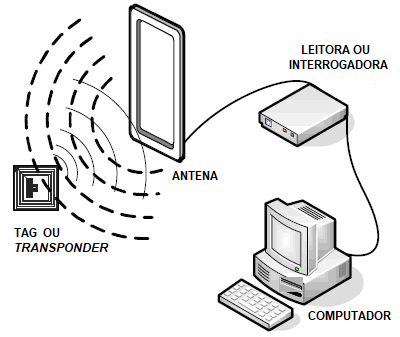
\includegraphics[width=0.6\linewidth]{figs/Fundamentos/Composicao.png}
    \caption{Composição básica de um sistema RFID. (Adaptado de EPC-RFID \cite{EPC-RFID-link})}
    \label{fig:ComposicaoRFID}
\end{figure}


As primeiras aplicações comerciais de RFID, como artigo eletrônico de vigilância (EAS - \textit{Electronic Article Surveillance}), aconteceram no final da década de 1960, desenvolvidas por empresas como: Kongo, Sensormatic (by Johnson Controls) e Checkpoint \cite{chawla2007overview}.

De acordo com Chawla e Ha \cite{chawla2007overview}, o sistema RFID consiste em leitoras e TAGS. A leitora tem como função se comunicar na faixa de alcance sem fio e coletar informações sobre os objetos aos quais as TAGS estão anexadas (ex.: entrada e saída de pessoas de um estabelecimento).

O funcionamento simplificado do RFID passivo pode ser observado na figura \ref{fig:DiagramaRFID}. Um gerador de sinais de radiofrequência (RF - \textit{radiofrequency}) emite um sinal à um transpônder com impedância variável e um codificador de identidade. O sinal emitido excita o oscilador presente na TAG,que por sua vez reflete o sinal modificado com as informações de identidade da TAG. O sinal de resposta é capturado por uma antena, amplificado e decodificado. A informação de identidade da TAG pode então ser processada, apresentada ou armazenada.

\begin{figure}[h]
    \centering
    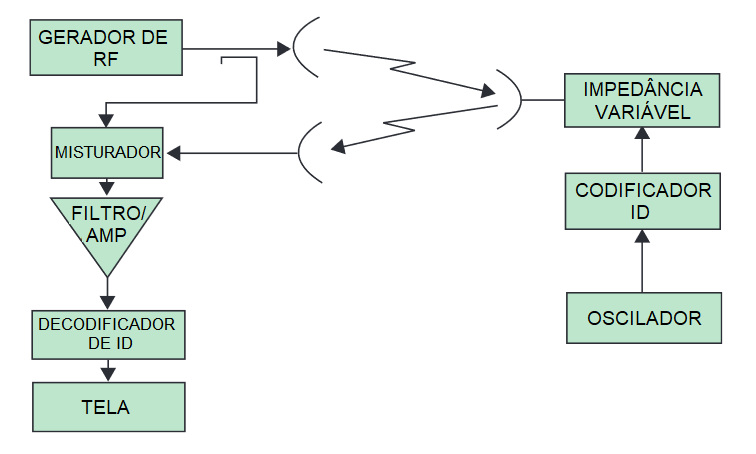
\includegraphics[width=0.6\linewidth]{figs/Fundamentos/RFIDdiagram.png}
    \caption{Diagrama de rede de uma comunicação RFID. (Adaptado de Landt, Jeremy \cite{landt2005history})}
    \label{fig:DiagramaRFID}
\end{figure}

A figura \ref{fig:DetalhesRFID} mostra os elementos internos dos dispositivos de um sistema RFID. Nela é possível observar o trajeto de dados da energização da bobina da TAG e envio de informação através da variação de potência do campo magnético. A energização alimenta o circuito da TAG que é composto de carga, codificador RF e chip de controle, memória e criptografia. O circuito excitado da TAG reflete o sinal codificado e é capturado pela bobina da antena da leitora, que interpreta o sinal e retransmite a informação em uma interface de rede para um computador.

\begin{figure}[h]
    \centering
    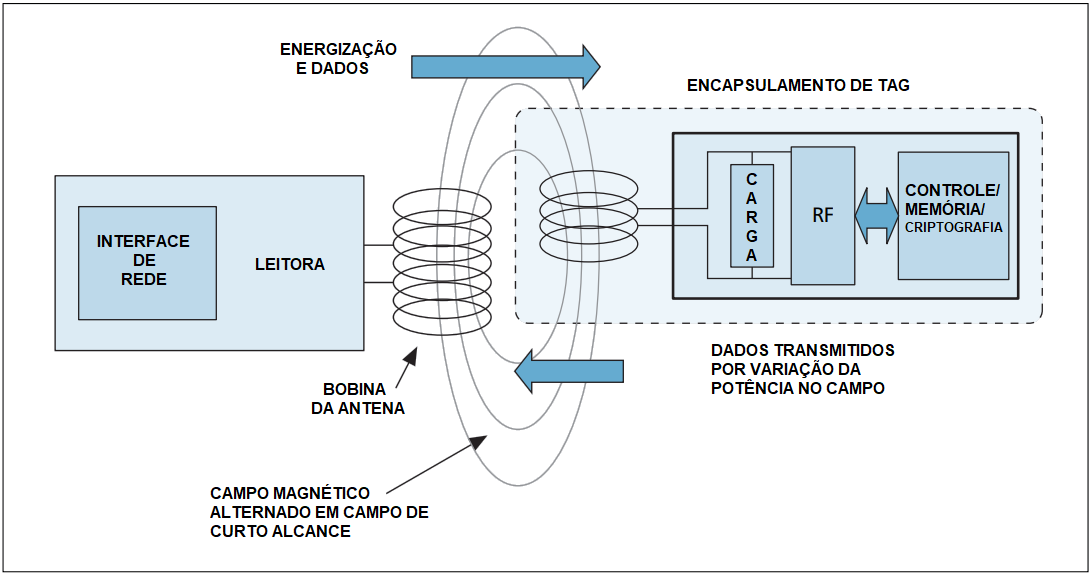
\includegraphics[width=0.8\linewidth]{figs/Fundamentos/RFIDdetails.png}
    \caption{Estrutura interna básica dos elementos de um sistema RFID. (Adaptado de Chawla e Ha \cite{chawla2007overview})}
    \label{fig:DetalhesRFID}
\end{figure}

\subsection{\textit{Middleware}} \label{section: middleware}

Chen et al. \cite{chenUsingRFID} define RFID como o conjunto de TAGs, leitoras, \textit{middleware} e sistema de aplicação, como pode ser visto na figura \ref{fig:RFID-Middleware}.

\begin{figure}[h]
    \centering
    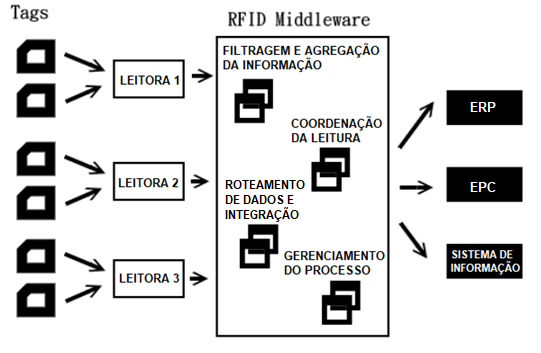
\includegraphics[width=0.6\linewidth]{figs/Fundamentos/RFID.png}
    \caption{Topologia de comunicação do \textit{middleware} RFID (Adaptado de Chen \textit{et al.} \cite{chenUsingRFID})}
    \label{fig:RFID-Middleware}
\end{figure}

\textit{Middleware} é o \textit{software} que liga o Sistema Operacional às aplicações. É comum definir um \textit{middleware} como um "encanamento" que leva dados de um ponto a outro. \cite{Middleware}

No caso do RFID, o \textit{middleware} é um \textit{software} que interpreta e organiza os dados enviados pelas leitoras. Ele realiza a filtragem e agregação da informação, a coordenação da leitura, o roteamento de dados e integração e o gerenciamento do processo. Ao final do processamento, ele disponibiliza os dados para aplicações que podem ser, por exemplo, ERPs (em inglês: \textit{Enterprise Resource Planning} - Planejamento de Recursos Empresariais), sistemas de informação ou um \textit{software} de localização de pessoas em ambientes fechados.

\subsection{RAIN RFID e IoT}

O padrão RAIN (acrônimo para \textit{RAdio frequency IdentificatioN} - Identificação por radiofrequência) é a união de diferentes tipos de \textit{hardware} e \textit{software} que possuem o propósito de ligar o meio RFID UHF com a computação em nuvem. É padronizada pela organização global de mesmo nome (RAIN) com o objetivo de popularizar o uso de RFID. \cite{RAIN}

RAIN RFID foi desenvolvido principalmente para aplicações de internet das coisas (IoT - \textit{Internet of things} em inglês). IoT é, segundo Gubbi, \textit{et al.} \cite{gubbi2013internet}:


\begin{quote}  
    "Interconexão de dispositivos de detecção e atuação, oferecendo a capacidade de compartilhar informações entre plataformas por meio de uma estrutura unificada, desenvolvendo uma imagem operacional comum para permitir aplicativos inovadores. Isso é conseguido através da detecção onipresente e contínua, análise de dados e representação de informações com a computação em nuvem como a estrutura unificadora." \cite{gubbi2013internet}
\end{quote}


\subsection{\textit{TAGs}}
TAGs, também conhecidas como transpônderes, são etiquetas ou chips microprocessadores de identificação. Esses dispositivos recebem sinal de rádio e transmitem, automaticamente, um sinal diferente. Cada TAG possui um número serial de identificação que a difere de outras. \cite{chawla2007overview}. Esses objetos podem armazenar informações como \textit{serial number} (número serial), \textit{model number} (número do modelo), bem como outras características como: data, cor, tamanho e preço. A TAG RFID é classificada de acordo com sua memória, tipo de comunicação e uso de energia, como é possível visualizar na tabela \ref{tab:comparativoTags}  \cite{AhmedIntegrationStreamMapping}.

 
\begin{table}[H]
\centering
\caption{Classificação de TAGs RFID (Adaptado de \cite{AhmedIntegrationStreamMapping})}
\label{tab:comparativoTags}
\begin{tabular}{p{3cm}p{9cm}}
\hline
\multicolumn{2}{c}{\cellcolor{lightgray}{Origem da alimentação elétrica}} \\ \hline
Passiva         &   Alimentada pela leitora através do próprio sinal de radiofrequência. Também chamada de 'reflexiva', 'alimentada por feixe' ou de 'retroespalhamento' (\textit{backscattering}).     \\ \hline
Semi-Passiva    &   Utiliza uma bateria para manter a memória na etiqueta ou alimentar os componentes eletrônicos que permitem que a etiqueta module o sinal refletido.    \\ \hline
Ativa           &   Alimentada por uma bateria interna. Possui maior alcance de leitura e é mais cara que as TAGs passivas. As baterias devem ser substituídas periodicamente.    \\ \hline
\multicolumn{2}{c}{\cellcolor{lightgray}{Tipo de Memória}} \\ \hline
Somente leitura       &   A memória é programada na fábrica e não pode ser modificada após sua fabricação. Geralmente armazena apenas 96 bits de informação.       \\ \hline
Leitura-escrita    &   A leitora RFID pode ler e escrever na memória desta TAG. É possível armazenar uma quantidade maior de dados (de 32 kb a 128 kb). É mais cara que os chips do tipo somente leitura.   \\ \hline
\multicolumn{2}{c}{\cellcolor{lightgray}{Tipo de Comunicação entre a TAG e a Leitora}} \\ \hline
Indução       &   Acoplamento eletromagnético ou indutivo de proximidade. Utilizada em Bandas de frequência LF e HF.       \\ \hline
Propagação    &   Propagação de ondas eletromagnéticas - campo distante. Opera nas faixas de frequência UHF e micro-ondas.   \\ \hline
\end{tabular}
\end{table}



É possível classificar as TAGs em três tipos, como pode ser visto na tabela \ref{tab:comparativoTags}: ativas, passivas e semi-passivas \cite{chawla2007overview}.  Existem vários tipos de TAGS ativas (alimentadas por baterias) e passivas, em várias faixas de frequência, presentes no mercado \cite{rao1999overview}. A Figura \ref{fig:tags-fundam} mostra exemplos de TAGS ativas e passivas.



\begin{figure}[h]
    \centering
    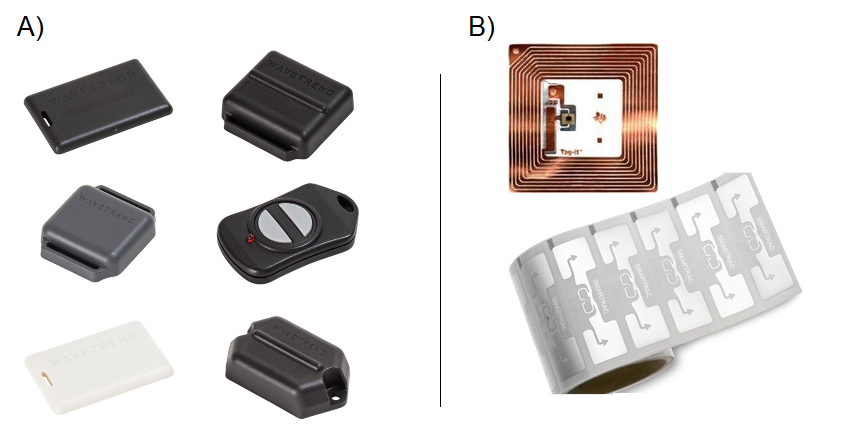
\includegraphics[width=0.8\linewidth]{figs/Fundamentos/tags.png}
    \caption{A) Exemplos de TAGs ativas \cite{wavetrend} - B) Exemplos de TAGs passivas \cite{IDTechEx} \cite{RFIDInsider}}
    \label{fig:tags-fundam}
\end{figure}





Segundo Rao \cite{rao1999overview}, TAGs ativas, como as apresentadas na figura \ref{fig:tags-fundam}A, tem como vantagem o alcance de distância de leitura maior do que as TAGs passivas, devido à sua construção com alimentação de energia própria. Como desvantagem, elas podem ser bem mais caras e exigem o uso de baterias \cite{rao1999overview}. Uma etiqueta RFID passiva, figura \ref{fig:tags-fundam}B, por sua vez, usará a energia das ondas de rádio do interrogador para retransmitir suas informações armazenadas de volta a ele \cite{EPC-RFID-link}.

As TAGs passivas podem possuir diversas construções de memória diferentes. O tipo mais simples é transpônder de 1-bit, muito utilizado em TAGs EAS (Artigo Eletrônico de segurança - \textit{Electronic Article Surveillance} em inglês). Ele possui um bit de memória apenas. O seu funcionamento é simples, a TAG responde ao interrogador um sinal de presença naquele ambiente, armazenando neste bit a informação de resposta, \textit{true} ou \textit{false}. \cite{book:klaus}

Já os transpônderes de n-bits podem possuir de poucos bits até 128 kb a depender do sistema. Eles se dividem em \textit{full-duplex}, \textit{half-duplex} e sequenciais. A diferença entre eles é o protocolo de comunicação entre a TAG e o interrogador. \cite{book:klaus}

\begin{itemize}
    \item \textit{Half-duplex}
    \begin{itemize}
        \item O interrogador alimenta o transpônder continuamente
        \item O interrogador e o transpônder se alternam para emitir dados de comunicação, com o transpônder utilizando frequências harmônicas para responder ao interrogador
    \end{itemize}
    \item \textit{Full-duplex}
    \begin{itemize}
        \item O interrogador alimenta o transpônder continuamente
        \item O interrogador e o transpônder emitem dados de comunicação simultaneamente, com o transpônder utilizando frequências subarmônicas e anarmônicas para responder ao interrogador
    \end{itemize}
    \item Sequencial
    \begin{itemize}
        \item O interrogador alimenta o transpônder somente durante a sua etapa de transmissão de dados;
        \item A transferência de dados do transpônder para a leitora ocorre somente durante curtos períodos de tempo, como uma resposta ao pulso de alimentação.
    \end{itemize}
\end{itemize}




\subsection{Antenas}

A antena é o equipamento de um sistema RFID capaz de perceber o sinal de uma TAG dentro de um determinado raio de cobertura. Elas se conectam às leitoras e são responsáveis por propagar os sinais enviados pela leitora no meio, energizar as etiquetas e escutar o sinal de resposta.

Antenas são dispositivos usados na transferência e captação de ondas eletromagnéticas em meios ilimitados no espaço. São projetadas em bandas de frequência de operação. Dessa forma, um sinal ou é atenuado ou é rejeitado por completo. \cite{antena}

\subsection{Efeitos causados por materiais e frequência de operação}

É amplamente conhecido na indústria do RFID e de outras tecnologias que trabalham com RF (radiofrequência - \textit{radiofrequency} em inglês) que os materiais presentes no ambiente onde se propagam os sinais transmitidos interferem com esse sinal.

Estudos com materiais mostram que podem existir nove tipos de perdas no sinal, como mostra Sanghera em seu livro\cite{book:SangheraRFID+}:
\begin{itemize}
    \item \textbf{Absorção:} Energia do sinal absorvida pelo meio;
    \item \textbf{Atenuação:} Diminuição da amplitude do sinal devido à absorção e dispersão;
    \item \textbf{Efeitos Dielétricos:} Capacidade do meio de reter carga. Gera atraso do sinal;
    \item \textbf{Difração:} "Dobra" de um sinal de radiofrequência ao atingir uma quina ou pequeno orifício;
    \item \textbf{Perda de espaço livre:} Diminuição da densidade do sinal devido à característica de propagação do sinal para todos os lados;
    \item \textbf{Interferência:} Ocorre no encontro de duas ondas de radiofrequência, pode ser construtiva ou destrutiva;
    \item \textbf{Reflexão:} Retorno do sinal em um ângulo isóceles ao de incidência em uma superfície plana. Geralmente ocorre no chão, teto e paredes;
    \item \textbf{Refração:} mudança de direção de trajetória do sinal, entretanto permeando o meio causador da refração;
    \item \textbf{Espalhamento:} Absorção e re-emissão do sinal, em direções aleatórias.
\end{itemize}
    
Sanghera mostra ainda uma tabela contendo a influência de cada material no sinal de radiofrequência \cite{book:SangheraRFID+} que é adaptada e apresentada a seguir (Tabela \ref{tab:InterfMateriais}).

\begin{table}[H]
\centering
\caption{Efeito dos materiais nos sinais de RFID (Adaptado de \cite{book:SangheraRFID+})}
\label{tab:InterfMateriais}
\begin{tabular}{p{5cm} p{7cm}}
\hline
\cellcolor{lightgray}{Material} & \cellcolor{lightgray}{Efeito no sinal RF}   \\ \hline
Papelão         &   Absorção        \\
Líquido condutivo    &   Absorção        \\
Vidro           &  Atenuação        \\
Conjunto de latas & Reflexão em múltiplas direções \\
Corpo humano ou animal & Absorção, dessintonização e reflexão \\ 
Metal & Reflexão \\
Plástico & Dessintonização devido ao efeito dielétrico \\ \hline
\end{tabular}
\end{table}

 Um estudo conduzido por Fletcher \cite{fletcher2005study} questiona, contudo, os efeitos dos sinais RF nos meios aquosos, e portanto, os efeitos no corpo humano e de animais por consequência. Ele afirma que, ao contrário do que se acredita, os líquidos interferem nas leituras dos sinais de RFID majoritariamente devido aos efeitos de reflexão e refração, enquanto o consenso é de que meios aquosos absorviam os sinais, principalmente.
 
 De uma forma ou de outra, as leituras RFID obtidas são de baixa qualidade quando os transpônderes ou as antenas estão próximas de meios aquosos ou pessoas e animais. Esse é o principal motivo de o monitoramento de localização por RFID, ou outras tecnologias RF, não possuir muita aderência para o propósito de monitorar pessoas enquanto a tecnologia avança a passos largos no monitoramento de produtos e aplicações de \textit{IoT}, visto que estes últimos são menos suscetíveis à perda de sinal.
 
 O livro de Thornton e Sanghera \cite{thornton2011cheat} mostra a influência causada pela escolha da frequência de funcionamento do sistema. Os protocolos RFID preveem o funcionamento da tecnologia em quatro faixas de frequência:
 
 \begin{itemize}
     \item Baixa frequência (LF - \textit{Low Frequency})
     \begin{itemize}
         \item opera a 125 kHz ou 134 kHz para dispositivos RFID
         \item Baixa distorção devido a água
         \item Curto alcance (até 10 cm)
         \item Utilizado para identificação de pessoas e animais à curta distância
     \end{itemize}
     \item Alta frequência (HF - \textit{High Frequency})
     \begin{itemize}
         \item opera a 13.56 MHz para dispositivos RFID
         \item alcance de até 3m
         \item sinal RF com comprimento de onda pequeno / baixa capacidade de penetração em materiais
         \item mais opções de velocidade de leitura em relação à baixa frequência
         \item utilizado em controle de acesso e rastreio de itens como bagagens
     \end{itemize}
     \item UHF (em inglês \textit{Ultra High Frequency} - Frequência Ultra Alta em tradução livre para o português)
     \begin{itemize}
         \item Diferentes frequências em diferentes países
         \begin{itemize}
             \item Faixa de 860-960MHz
             \item 902-928MHz no Brasil (geralmente 915MHz)
         \end{itemize}
         \item alta distorção devido a água
         \item a frequência de operação depende do país onde o equipamento é homologado
         \item maior alcance que LF e HF
         \item usado para gerenciamento de estoque e armazéns
     \end{itemize}
     \item Micro-ondas
     \begin{itemize}
         \item Faixa de 2,44-5,80GHz para dispositivos RFID
         \item Alta velocidade de leitura
         \item Longo alcance
         \item baixo desempenho próximo a água
         \item utilizado para identificação de veículos e \textit{supply chain} (em português, "cadeia de suprimentos" ou "cadeia de logística")
     \end{itemize}
 \end{itemize}


A imagem \ref{fig:impactoFrec} de Oliveira e Rocha \cite{TG2013OliveiraERocha}, traduzida da original no livro de Thornton e Sanghera \cite{thornton2011cheat}, simplifica os conceitos do impacto da frequência de operação no sinal RFID.

\begin{figure}[H]
    \centering
    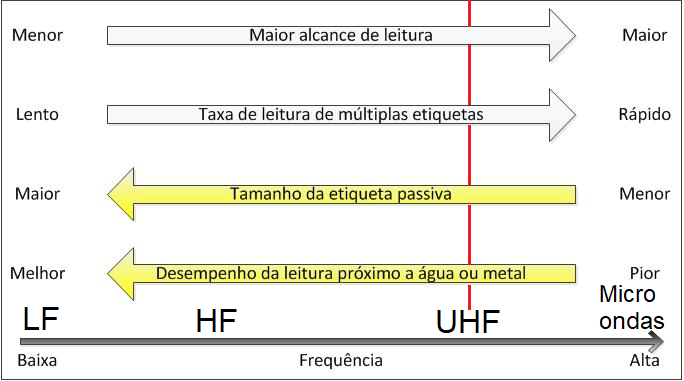
\includegraphics[width=0.8\linewidth]{figs/Fundamentos/frequencia.png}
    \caption{Impacto da frequência de operação nas leituras RFID. (Adaptado de \cite{TG2013OliveiraERocha} e \cite{thornton2011cheat})}
    \label{fig:impactoFrec}
\end{figure}

A caracterização do sistema e das etiquetas passivas utilizados pode ser caracterizada na porção mais à direita do gráfico da figura \ref{fig:impactoFrec}, por se tratar de um sistema UFH, o que indica que as TAGs não necessitam de um tamanho exageradamente grande, e que o alcance do sistema é maior.

O gráfico da figura \ref{fig:impactoFrec} pode ser analisado alocando os sistemas LF à esquerda, onde o alcance é menor e o desempenho próximo à água e metais é melhor, progredindo para a direita na ordem: HF, UHF e micro ondas. A cada progressão de banda de frequência, o alcance do sistema é aprimorado à custa do desempenho quando próximo de materiais problemáticos para sinais RF.

\subsection{RSSI}

O Indicador de Intensidade do Sinal Recebido (\textit{Received Signal Strength Indication}), em poucas palavras, é a medida de quão eficiente um dispositivo pode ser na detecção de um sinal/ruído.

Segundo Buffi \cite{buffi2018rssi}, existem duas impedâncias intrínsecas à cada TAG que geralmente correspondem à carga de impedância correspondente ($Z_{CM}$) e uma carga de impedância de curto-circuito ($Z_{SC}$). Durante a comunicação entre a leitora RFID e a TAG alterna-se entre as duas impedâncias, como mostra a figura \ref{fig:rssiFUND}.

\begin{figure}[H]
    \centering
    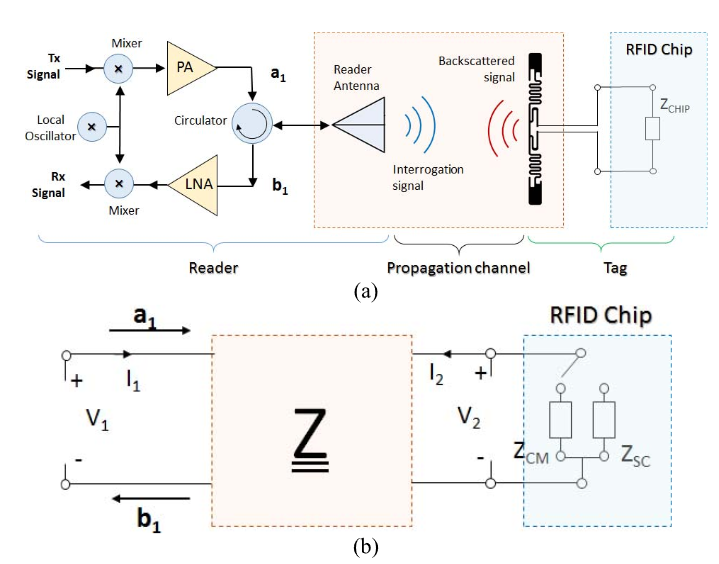
\includegraphics[width=0.8\linewidth]{figs/Fundamentos/rssi.PNG}
    \caption{(a) Representação esquemática de uma TAG equipada com uma antena, um chip RFID e um leitor, este último constituído por uma antena, um circulador, um amplificador de potência para o sinal transmitido e amplificador de baixo ruído para o sinal recebido. (b) Matriz de impedância equivalente que representa a antena do leitor, a antena do TAG e o canal de propagação entre elas. Para gerar um \textit{backscattering} modulado, a antena da TAG é conectada a uma carga de impedância combinada conjugada ($Z_{CM}$) ou a um curto-circuito ($Z_{SC}$). \cite{buffi2018rssi}}
    \label{fig:rssiFUND}
\end{figure}

O sinal RSSI é calculado a partir do módulo da diferença dos coeficientes de refração $\Gamma$ as amplitudes do sinal enviado e do sinal recebido, como mostra a equação \ref{eq:rssiFUNDa}. 

\begin{equation}
    RSSI = k {|\Gamma_{CM}(x,y) - \Gamma_{SC}(x,y)|}^2
    \label{eq:rssiFUNDa}
\end{equation}

Na equação \ref{eq:rssiFUNDa} $k$ representa uma constante, $x$ e $y$ representam as coordenadas da TAG em relação à leitora, e $\Gamma_{CM}$ e $\Gamma_{SC}$ representam os coeficientes de refração do sinal de retorno. O coeficiente $\Gamma$ é proporcional à relação entre as amplitudes do sinal enviado pela leitora e pelo sinal de retorno da TAG lido pela antena, de acordo com a equação \ref{eq:rssiFUNDb}.

\begin{equation}
    \Gamma = \frac{b_1}{a_1}
    \label{eq:rssiFUNDb}
\end{equation}

Na equação \ref{eq:rssiFUNDb} $a_1$ é a amplitude do sinal enviado pela leitora e $b_1$ é a amplitude do sinal de resposta capturado pela antena.

As equações \ref{eq:rssiFUNDa} e \ref{eq:rssiFUNDb} discutidas nesta seção são apresentadas para informar o leitor da origem e dos cálculos feitos internamente pela leitora Impinj \textit{Speedway} R420, modelo utilizado neste trabalho e apresentado na seção \ref{section:met-leitora}. Estes cálculos são feitos diretamente em \textit{hardware} e tratados no \textit{middleware} da leitora e, portanto, não se executam tais cálculos neste trabalho. As informações de RSSI são adquiridas diretamente da leitora para uso do programa criado neste trabalho.
    
\section{Rede de Petri}
    
A Rede de Petri consiste em uma ferramenta gráfica e matemática que possui inúmeras aplicações. Segundo Francês \cite{Frances}, a representação gráfica básica de uma rede de Petri compreende dois componentes principais: um ativo (transição) - que graficamente é uma barra - e um passivo (lugar), graficamente representado pelo círculo. 

Algumas de suas aplicações são a de avaliar desempenhos, possibilitar a concepção de software em tempo real e/ou distribuído, avaliar o gerenciamento bases de dados, interfaces homem-máquina, atuar em sistemas de informação, controle, logística e transporte, além de outras inúmeras funcionalidades. As vantagens do uso podem ser descritas brevemente a seguir: \cite{Cardoso1997}

\begin{itemize}
    \item descrição de ordem parcial em eventos, possibilitando avaliar a flexibilidade;
    \item representação explícita dos estados;
    \item facilitação nos níveis da estrutura hierárquica do controle;
    \item utilização de uma única família de ferramentas; 
    \item descrição precisa e formal das sincronizações, garantindo a segurança do funcionamento;
\end{itemize}
    
\section{Efeito Doppler} \label{section:doppler_fund}

O Efeito Doppler ocorre quando ondas são emitidas ou refletidas por um objeto em movimento. É um fenômeno físico importante para a análise da detecção de sinais em movimento.

As leitoras de RFID geralmente possuem capacidade de calcular o desvio de fase do sinal de resposta de \textit{backscatter} das TAGs, de acordo com a equação \ref{eq:desvioFase}. A partir dessa informação, é possível obter o valor da frequência Dopler causada pelo deslocamento da TAG. \cite{nikitin2010phase} \cite{tesch2015rfid}

\begin{equation}
    \theta = \theta_{Prop} + \theta_{o} + \theta_{BS}
    \label{eq:desvioFase}
\end{equation}

Na equação \ref{eq:desvioFase} $\theta$ representa a fase do sinal recebido da TAG, $\theta_{Prop}$ é a fase acumulada devido à propagação de ondas eletromagnéticas, $\theta_{o}$ é o deslocamento de fase (\textit{offset}) nos cabos e antenas e $\theta_{BS}$ é a fase de retroespalhamento (\textit{backscatter}) da modulação de TAG. \cite{nikitin2010phase} \cite{tesch2015rfid}

As leitoras RFID utilizam a fase do sinal de retorno $\theta$ para calcular a frequência Doppler através da equação \ref{eq:Doppler} a seguir.\cite{tesch2015rfid}

\begin{equation}
    f_D = \frac{\Delta \theta}{4 \pi \Delta T}
    \label{eq:Doppler}
\end{equation}

Na equação \ref{eq:Doppler} $f_D$ é a frequência Doppler. Os valores de $\Delta \theta$ e $\Delta T$ podem ser obtidos com as equações \ref{eq:deltaTheta} e \ref{eq:DetaTe}, respectivamente.\cite{tesch2015rfid}

\begin{equation}
    \Delta \theta = \theta_2 - \theta_1
    \label{eq:deltaTheta}
\end{equation}

\begin{equation}
    \Delta t = t_2 - t_1
    \label{eq:DetaTe}
\end{equation}

Na equação \ref{eq:deltaTheta}, $\theta_1$ e $\theta_2$ são as leituras de fase da TAG nas posições iniciais e finais de leitura, calculados a partir da equação \ref{eq:desvioFase}, como pode ser visualizado na figura \ref{fig:dopplerFund}. Na equação \ref{eq:DetaTe}, $t_1$ e $t_2$ correspondem aos tempos das leituras de $\theta_1$ e $\theta_2$ da equação \ref{eq:deltaTheta}. \cite{tesch2015rfid}

\begin{figure}[H]
    \centering
    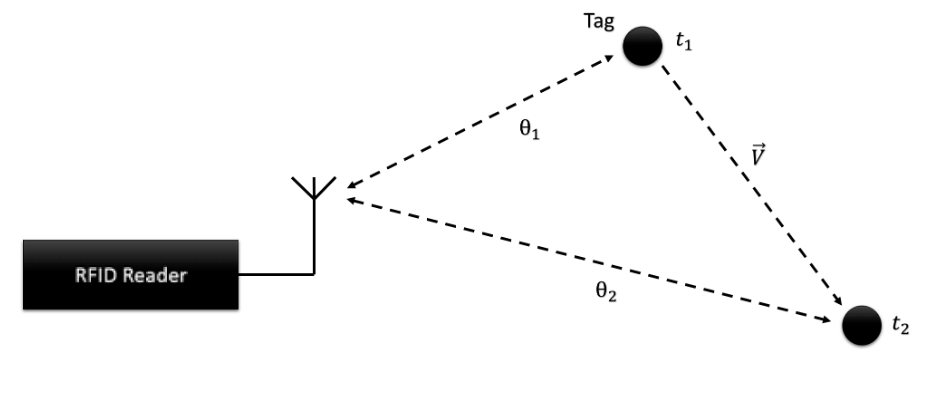
\includegraphics[width=0.8\linewidth]{figs/Fundamentos/doppler.PNG}
    \caption{Frequência Doppler calculada a partir da fase do sinal de retorno da TAG \cite{tesch2015rfid}}
    \label{fig:dopplerFund}
\end{figure}

A figura \ref{fig:dopplerFund} mostra uma TAG em duas posições espaciais diferentes, em tempos $t_1$ e $t_2$ diferentes. Em cada posição o sinal de leitura retorna à antena com uma fase $\theta$ diferente.

Assim como o valor de RSSI, o valor de frequência de efeito Doppler é calculado internamente em \textit{hardware} e \textit{middleware} da leitora Impinj \textit{Speedway} R420. Não será calculada a frequência Doppler neste trabalho, sendo que as leituras realizadas pelo equipamento utilizado já informam, juntamente às outras informações da TAG (número EPD e valor RSSI), o valor de frequência Doppler.
    
\section{Localização \textit{indoor}}

O rastreio e localização de pessoas em ambientes fechados é algo fortemente desejado desde o surgimento das tecnologias de localização por sinais de radiofrequência. É imaginado um futuro onde equipes de segurança saibam exatamente onde resgatar uma pessoa com dificuldades, dentro de um edifício; sistemas de ar-condicionado dimensionam automaticamente as suas potências baseados na ocupação do local aumentando a eficiência energética; mapas de ambientes fechados públicos que indicam o caminho até o destino final interno.

A localização de pessoas e objetos já está muito avançada para ambientes externos, com exemplos de muito sucesso como o sistema de posicionamento global - GPS (\textit{Global Positioning System} em inglês) e seus similares (Galileo, Glonass, Compass), e também do Cell-ID - tecnologia de localização de dispositivos GSM/WCDMA/CDMA por triangulação de torres de celular. Contudo, a localização em ambientes fechados ainda é muito restrita, principalmente devido às restrições de comunicação por sinais RF em ambientes passíveis de obstrução por objetos e fontes de reflexão e demais tipos de interferência. Problemas como a atenuação e dispersão do sinal, sinais duplos ou múltiplos, e a grande quantidade de dispositivos comunicando-se em um pequeno espaço em algumas aplicações (o que gera conflito de diversas tentativas de estabelecimento de comunicação ao mesmo tempo), dificultam o desenvolvimento de uma tecnologia definitiva para esta aplicação.

Para desviar dos empecilho, soluções específicas para diversas aplicações são criadas. A indústria larga na frente, com sistemas de rastreio e posicionamento de produtos e equipamentos, como em armazéns e linhas de produção. O comércio também já possui soluções para prevenção de perdas e roubos, e começa a aplicar os conceitos de rastreamento de produtos de armazéns para identificar roupas e sapatos em estantes, por exemplo. A área de soluções para cidades pesquisa tecnologias IoT.

A área de localização de pessoas em ambientes fechados possui pesquisas com diversas tecnologias, como WiFi, Bluetooth, GSM, Radiação Infravermelha, processamento de imagens, RFID ativo e passivo, entre outras. Todas possuem vantagens e desvantagens.

A grande diferença entre as técnicas de rastreamento do RFID ativo e passivo é que, geralmente, as propostas com RFID ativo utilizam algum tipo de triangulação de sinais, com um transpônder e diversas leitoras \cite{bouet2008rfid} \cite{jin2006indoor} \cite{sanpechuda2008review}, devido às características de funcionamento desse sistema. As estratégias com RFID passivo costumam necessitar de pontos de interrogação e controle de acesso para funcionar, devido ao curto alcance da maioria dos sistemas. Entretanto, algumas aplicações funcionais de localização cartesiana recentes utilizando frequências mais altas como UHF e Microondas \cite{xarray} mostram que é possível minimizar as dificuldades de implementar sistemas de localização com RFID passivo.

Algumas implementações, como a de Tesoriero \textit{et al.} \cite{tesoriero2008using}, inovam ao misturar sensores ativos e passivos. Sua pesquisa apresenta o ambiente de um museu, onde os visitantes carregam PDAs (Assistentes Pessoais Digitais - em inglês \textit{Personal Digital Assistants} que são leitoras RFID passivo, e as TAGs marcam os locais e as obras, invertendo o papel padrão dos elementos, e criando um mapa do museu a partir do posicionamento das TAGs.

Utilizando os recursos disponíveis na UnB e no LARA, este trabalho propõe uma solução própria, que será explanada no capítulo \ref{chap:Metodos} - Metodologia.



\section{Cálculo de taxa de amostragem}

A fabricante das leitoras relata a relação do modo de leitura definido na figura \ref{fig:readermode_settings} com a frequência de identificação dos cartões. Segundo a Impinj \cite{reader_mode}, o modo \textit{"DenseReaderM8"} leva oito ciclos para processar cada bit de leitura, como pode ser visto na figura \ref{fig:modulation}. Considerando que a leitora funcione à taxa de 900MHz, arredondando os valores reais de frequência de operação, realizam-se os cálculos da equação \ref{eq:taxadeamostragem} para calcular o menor tempo possível de período de leitura.

 \begin{figure}[H]
    \centering
    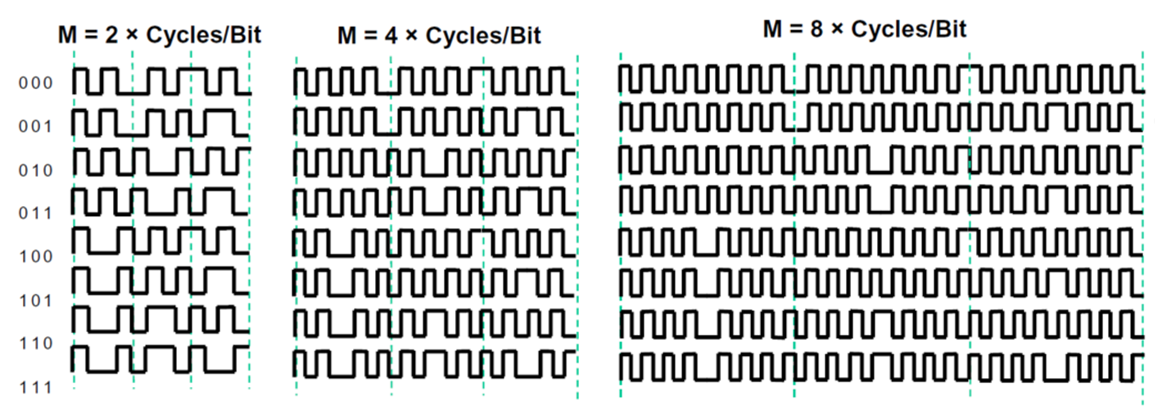
\includegraphics[width=0.8\linewidth]{figs/Metodologia/modulation.png}
    \caption{Modulação de modos de leitura \cite{reader_mode}}
    \label{fig:modulation}
\end{figure}

\begin{equation}
    T_A = \frac{1}{f_{op}}*M*B*C
    \label{eq:taxadeamostragem}
\end{equation}

Na equação \ref{eq:taxadeamostragem}, a variável $T_A$ representa o período de amostragem mínimo, $f_{op}$ é a frequência de operação, $M$ é o modo de leitura (quantos ciclos por bit são necessários), $M$ é o número de Miller \cite{reader_mode}, que registra o numero de ciclos por Bit lido, $B$ é o número de Bits total do chip da TAG e $C$ é uma constante que relaciona o atraso na leitura provocada por existirem múltiplas TAGs no campo de cobertura da antena. Realizando os cálculos para o caso específico deste trabalho, obtém-se o valor calculado na equação \ref{eq:amostragem2}.

Os valores de taxa de amostragem serão calculados na seção \ref{section:amostragem}.

